\section{Results}

\subsection{Step-by-step Example with OR}
Recall the two bit function OR which returns $1$ if there
is at least one $1$ in the input and returns $0$ otherwise.
To understand Reichardt's formulation and our conversion
to Boyd's standard form, consider as inputs to our tool
the case with function $f: D \rightarrow E$ where
$D \subseteq {\{0,1\}}^2$ and $E =\{OR(x): x \in D \}$.
Let $F$ be the set of $(y,z)$ such that $f(y) \neq f(z)$. In this
case, $F = \{(00,01), (00,10), (00,11), (01,00), (10,00), (11,00)\}$

Our matrix $\X$ will be created as follows:
\begin{align}
\X = \begin{blockarray}{ccccc}
\qquad & 00 & 01 & 10 & 11 \\
\begin{block}{c[cccc]}
  00 & X_{(00,00)} & X_{(00,01)} & X_{(00,10)} & X_{(00,11)}\\
  01 & X_{(01,00)} & X_{(01,01)} & X_{(01,10)} & X_{(01,11)}\\
  10 & X_{(10,00)} & X_{(10,01)} & X_{(10,10)} & X_{(10,11)}\\
  11 & X_{(11,00)} & X_{(11,01)} & X_{(11,10)} & X_{(11,11)}\\
\end{block}
\end{blockarray} \nonumber 
\end{align}


The objective function of the SDP is:
\begin{align} \label{eq:reichardtObj} 
    f_{\text{bound}} &= M(\X) = \max_{y \in D} \sum_{j \in [n]}
    \bra{y,j}\X\ket{y,j} \nonumber \\
    &= \max\{ \tr{X_{(00,00)}}, \tr{X_{(01,01)}}, \tr{X_{(10,10)}}, \tr{X_{(11,11)}} \} \nonumber
\end{align}
subject to constraints
\begin{align}
    \X \succcurlyeq 0  \nonumber 
\end{align}
and
\begin{align}
    \forall (y,z) \in F \sum_{j \in [n]: y_j \ne z_j} 
    \bra{y,j} \X \ket{z, j} = 1. \nonumber 
\end{align}
Which is equivalent to:
\begin{align}
    \tr{X_{(00,01)}} &= \tr{X_{(00,10)}} = \tr{X_{(00,11)}} = 1 \nonumber \\
    \tr{X_{(01,00)}} &= \tr{X_{(10,00)}} = \tr{X_{(11,00)}} = 1 \nonumber
\end{align}

Our goal is to minimize $M$, and thus $f_{\text{bound}}$ by finding the optimal value of $\X$.

To make use of this definition, it's helpful to convert
the problem into a more canonical form to make use of algorithms published to solve SDP's. We convert Reichardt's problem 
to Boyd's standard form as shown below \cite{boyd2004convex}:
\begin{align}\label{Eq:boyd_obj}
    M(\X) = \tr(C\X) 
\end{align}
subject to
\begin{align} \label{Eq:boydSemi}
    \X \succcurlyeq 0   
\end{align}
and for $i \in \{1,...,p\}$
\begin{align} \label{Eq:boydTraceCon}
    \tr(A_i \X) = b_i. 
\end{align}
where $A_i$ and $C$ are matrices and $b_i$ is a scalar for each $i$.

Given the function $f$ and input size $n$,
we can define our set of matrices
and scalars $A_i$, $b_i$, and $C$ such that these two
problems are equivalent. We can then use developed algorithms to solve the problem and obtain our optimal bound on quantum query complexity for the function $f$.

We begin our conversion by examining the formulation of Reichardt's definition. 
$\X$ contains chunks of size 
$n \times n$, each corresponding to an element of the Cartesian product 
$D \times D$. Each axis of the matrix is partitioned into $|D| = 2^n$ 
equal parts such that we have chunks on the interior of the matrix 
corresponding to ordered pairs of inputs. Each chunk is of 
size $n \times n$ as mentioned previously so $\X$ is an 
$n2^n \times n2^n$ matrix. Below we consider $\X$ of the 
OR function with one bit inputs:
\begin{align}
\X = \begin{blockarray}{ccc}
\qquad & 0 & 1 \\
\begin{block}{c[cc]}
  0 & X_{(0,0)} & X_{(0,1)} \\
  1 & X_{(1,0)} & X_{(1,1)} \\
\end{block}
\end{blockarray}
\end{align}

In this instance, each sub-matrix $X_{(i,j)}$ is a $ 1
\times 1 $ matrix. This is the same construction used for
each input size $n$ where there is a sub-matrix
corresponding to every ordered pair of inputs in $D$.

To convert Reichardt's form into an
equivalent SDP in standard form, we first convert the
constraints and then the objective function. It's clear
that constraints in \cref{Eq:reichardtSemi} and 
\cref{Eq:boydSemi} are equivalent, simply requiring that
$\X$ is positive semidefinite.

The second constraint in Reichardt's form requires that
given a sub-matrix corresponding to a pair of inputs with
different outputs, the elements on this sub-matrix's
diagonal corresponding to bits that differ in the two
input strings sum to $1$. For each element in $F$, we can
define a matrix $A_i$ that moves the correct elements of
the corresponding sub-matrix's diagonal to the diagonal
of $A_i \X$ and sets other diagonal entries of $A_i \X$
to zero. In this way the trace of $A_i \X$ is equal to
the sum in \cref{Eq:reichardtOffDiag}. Therefore we set
each $b_i$ to $1$ to make the constraints equivalent.


For example, consider a matrix $X$ where
\begin{align}
    X = \left[ \begin{matrix} 1 & 2 \\ 3 & 4 \end{matrix} \right] \nonumber
\end{align}
and suppose we want to put the top right value $2$ on the diagonal.
We could define $A$ as below:

\begin{align}
    A = \left[ \begin{matrix} 0 & 0 \\ 1 & 0 \end{matrix} \right] \nonumber
\end{align}

Therefore,
\begin{align}
    A \cdot X = \left[ \begin{matrix} 2 & 0 \\ 4 & 0 \end{matrix} \right] \nonumber
\end{align}
and subsequently,
\begin{align}
    \tr(A \cdot X) = 2. \nonumber
\end{align}

Through a similar construction we can build our set of
matrices $A_i$ for each element of $F$ where we set $b_i
= 1$. Having now created $A_i$ and $b_i$ for $i = 1,2,..., |F|$, 
we have defined constraints equivalent to \cref{Eq:reichardtSemi}
and \cref{Eq:reichardtOffDiag}, thus creating an SDP 
in Boyd's form that is equivalent to the SDP in Reichardt's.

The problem is now that \cref{Eq:boyd_obj}
does not have a maximum in the way \cref{eq:reichardtObj}
requires. Our solution is to convert this maximum to a
linear function by introducing slack variables. We 
construct a new $\mathcal{X}$ from our original $\X$,
\begin{align}
    \Xb =
    \left[
    \begin{matrix}
    \X & 0 \\
    0 & S
    \end{matrix}
    \right] \nonumber
\end{align}
%\begin{equation}
%    \Xb = \left[\begin{matrix} \X \cdots \cdots 0 \\
%                                \vdots \ddots \vdots \\
%                                0 \cdots \cdots z  \end{matrix}
%                                \right]  
%\end{equation}
where $S$ is a diagonal matrix
with objective function $z$ in the bottom right most entry
and slack variables $s_i$ for $i \in [|D|]$
along the rest of the diagonal.

We guarantee that $z$ is the maximum
diagonal chunk of $\X$
by generating another set of matrices 
$\Ap_i$ and scalars $\bp_i$ for $i \in [|D|]$
where $\bp_i = 0$.
For each element of $D$, define a $c_i$ such that
\begin{align}
    c_i = \sum_{j \in [n]} \bra{y,j}\X\ket{y,j}
    \nonumber
\end{align} 
where $y$ is the $i^{th}$ element of $D$, making $c_i$ equivalent to the trace of the corresponding sub-matrix on the diagonal of $\X$.
Our goal is to enforce that $z$ is the maximum $c_i$.
By requiring that $s_i + c_i = z$ and using
the fact that $s_i$ is positive
($\Xb$ is semidefinite so $S$ is as well),
we can keep $z$ larger than or equal to $c_i$.
The semidefinite program minimizes $z$
by our choice of $C$ so $z$ meets the maximum $c_i$.

To enforce $s_i + c_i = z$, define $\Ap_i$ as a diagonal
matrix  with 1s along the chunk
corresponding to the $i^{th}$ input,
1 in the entry corresponding to $s_i$,
and -1 in the entry corresponding to $z$.
In a slight abuse of notation, we show an example
of $\Xb A_i$.
\begin{align}
\left[\begin{matrix} c_i & 0 & 0 \\
                    0 & s_i & 0 \\
                    0 & 0 & z \end{matrix} \right]
\left[\begin{matrix} 1 & 0 & 0 \\
                    0 & 1 & 0 \\
                    0 & 0 & -1 \end{matrix} \right]
= \left[\begin{matrix} c_i & 0 & 0 \\
                    0 & s_i & 0 \\
                    0 & 0 & -z \end{matrix} \right]
            \nonumber
\end{align}
Notice that the trace of $\Xb A_i$
is $c_i + s_i - z$.
By setting $\bp_i = 0$, we have that $z$ is
greater than or equal to $c_i$.

The final matrix we define is $C$.
Our goal is to extract $z$ from $\Xb$
so $C$ has a single non-zero value in the 
entry corresponding to $z$.
\begin{align}
    C = \left[\begin{matrix} 0  \cdots 0 \\
                                \vdots \ddots \vdots \\
                                0 \cdots  1  \end{matrix}
                                \right]  
                                \nonumber
\end{align}

We will now prove that using our construction,
$z = \max\{c_1, c_2, ... c_{|D|}\}$ in the optimal $\Xb$

\todo{make formal "theorem"}

Notice that because our matrix $\Xb$ is semidefinite 
and diagonal, all of its diagonal entries are non-negative. 
Assume for contradiction that $z < c_i$
for some $i \in \{1,2,..., |D|\}$.
Therefore $z < c_i + s_i$ since $s_i \geq 0$.

By our constraint, $z = c_i + s_i$, 
meaning that $z < z$, a contradiction! 
Therefore it must be the case that $z$ is an 
upper bound of the traces of our sub-matrices $c_i$. 

Now assume for contradiction that $z \ne  \max\{c_1, c_2, ...
c_{|D|}\}$. We know that $z$ is an upper bound so we only need to
show that there is no upper bound of this finite set that is less
than $z$ to show it is the maximum. Our assumption is equivalent to
the statement that there does not exist a constant $a$ such that $a
> c_i \forall i$ and $a < z$. If $a$ did exist, then there would
exist an $\Xb$ that also satisfies all of our constraints,
but with $a$ in the bottom right most entry instead of $z$. This
would mean that our objective function was improved over our
initial matrix as $a < z$, meaning that the $\Xb$ we found
is not optimal: a contradiction. We conclude that our constraints
are equivalent to those outlined by Reichardt, while matching the
form of Boyd.

Once given a function $f$ and all possible inputs to the
function of length $n$ ($D$), we can then define matrices
$C, A_i, \Ap_i$ and vectors $b_i, \bp_i$ such that the solution of Boyd's SDP
produces the solution of the Reichardt's SDP which
produces the optimal bound of quantum query complexity for
arbitrary Boolean functions.

\todo{step by step example with OR}

Given sets $D$ and $E$ such that
$f : D \rightarrow E$ for $f$ a Boolean function,
we construct matrices corresponding to the constraints
in \cref{Eq:boyd_obj}.
Our implementation uses Python3 and the NumPy library \cite{numpy}.
We build $A_i$ for $i \in [|F|]$ to enforce the condition
outlined in \cref{Eq:reichardtOffDiag} and set $b_i=1$.
We build $\Ap_i$ for $i \in [|D|]$ to enforce
that $z$ is the maximum $c_i$ and set $\bp_i = 0$.
Finally, we build $C$ to select $z$ from $\Xb$. To solve the SDP with our constraints,
we implemented Wen et al.'s ADM algorithm.



So far we have illustrated the SDP and its solution
through the example of the OR function.
Recall that OR takes as input $n$ bit strings
and returns 0 if there are no 1s in the input
and 1 otherwise.
We extend our analysis of OR by illustrating
an application of our SDP solver.

\begin{figure}[ht]
\centering
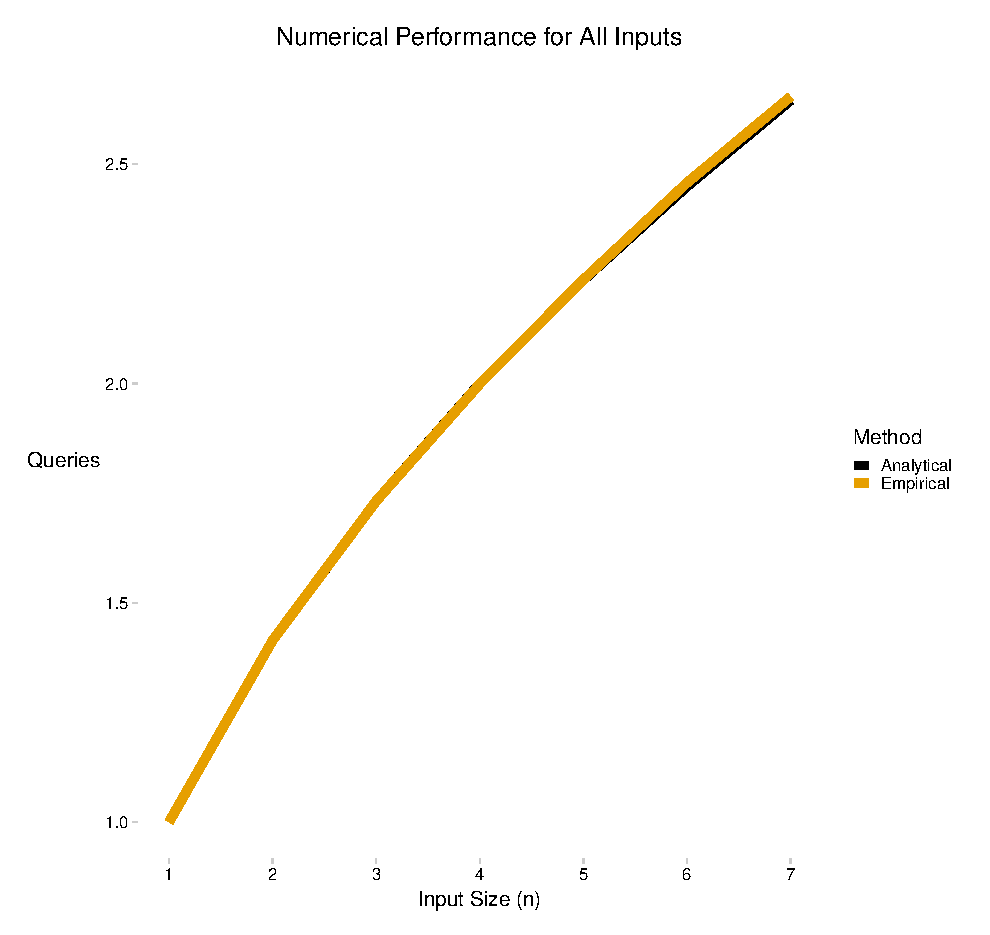
\includegraphics[scale=.5]{figure_all_or_complexity}
\caption{The proven analytical optimal query complexity
and calculated empirical optimal query complexity by 
size of input bit string.}
\label{fig:or_all_complexity}
\end{figure}

\begin{figure}[ht]
\centering
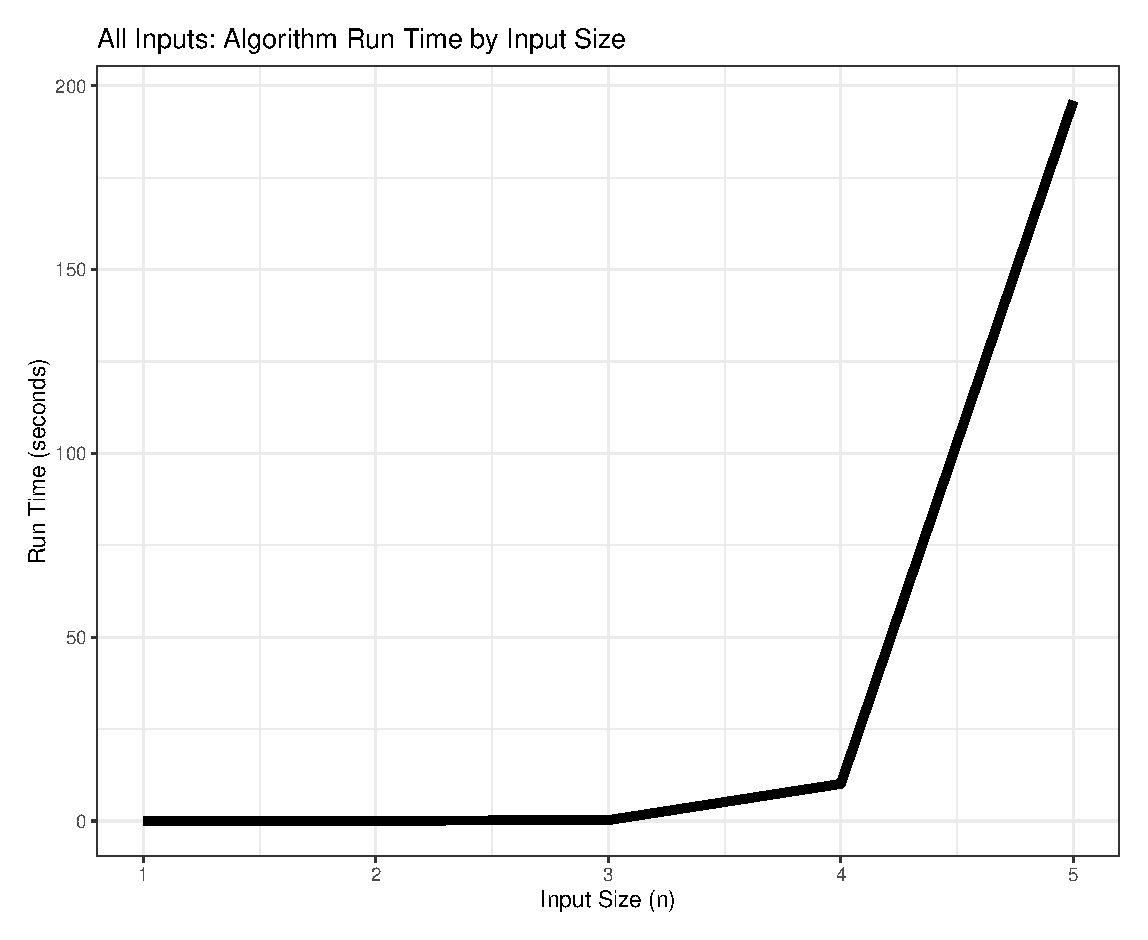
\includegraphics[scale=.4]{figure_all_or_time}
\caption{runtime of SDP solver by size of input strings.}
\label{fig:or_all_runtime}
\end{figure}

\subsection{OR Function: Worst-case Boolean Inputs}\label{sec:speed}
In \cref{fig:or_all_complexity}, we see that our algorithm
correctly calculates the optimal query complexity of the OR function.
(The analytical and empirical lines are so close that one
is mostly obscured).
In \cref{fig:or_all_runtime}, we see that the runtime grows
exponentially with respect to input size $n$.

Our algorithm's performance is displayed in \cref{fig:or_all_runtime}.
We see that runtime grows exponentially with respect to input size as expected, 
given the exponential increase in the cardinality of the set $D$ of all
inputs of length $n$. 
We also see that our algorithm is accurately calculating the
optimal quantum query complexity of the OR function. 

Using the known results of the quantum query
complexity of the OR function along with our
algorithm's performance in regard to the known
optimal values, we believe that our algorithm is
correct. Proof's of the algorithm's mathematical
correctness can be found in Wen et. al. Proof of the
algorithm's is shown through these results as well as
review of our code posted on GitHub. Knowing that our
algorithm is correct, we can then proceed to improve
it in several ways. 

First, we can attempt to improve runtime while
maintaining the correctness of the algorithm. Later,
we might be able to alter the algorithm
mathematically to take advantage of the structure
given in SDP's formed from quantum algorithms. 
It has also been claimed that the dual of this semidefinite
programming problem yields the quantum algorithm with minimal query complexity.
However, this optimal solution to the dual may not be easily 
interpreted as an algorithm as there could be many optimal, feasible solutions. 
Semidefinite programming problems also don't guarantee the tightness of the dual,
as is the case in linear programming. 
These problems all pose potential areas of future expansion.

\subsection{OR Function: All Boolean Inputs}

A simple approach to speeding up the runtime of our
algorithm is to simply decrease the number of input
strings considered for a given input size $n$. It's
important that we still obtain a good approximation
of the correct answer, so we need to ensure that the
inputs we do analyze will lead to the correct result.
Because the bounds of our algorithm are adversarial,
meaning that they are worst-case bounds, we can opt
to only use the worst-case inputs.

Again returning to our OR example, the hardest inputs are
either entirely zeros, or contain only a single 1. 
Using these inputs, we can then run our algorithm to 
compare both runtime and precision of results.

\begin{figure}[ht]
\centering
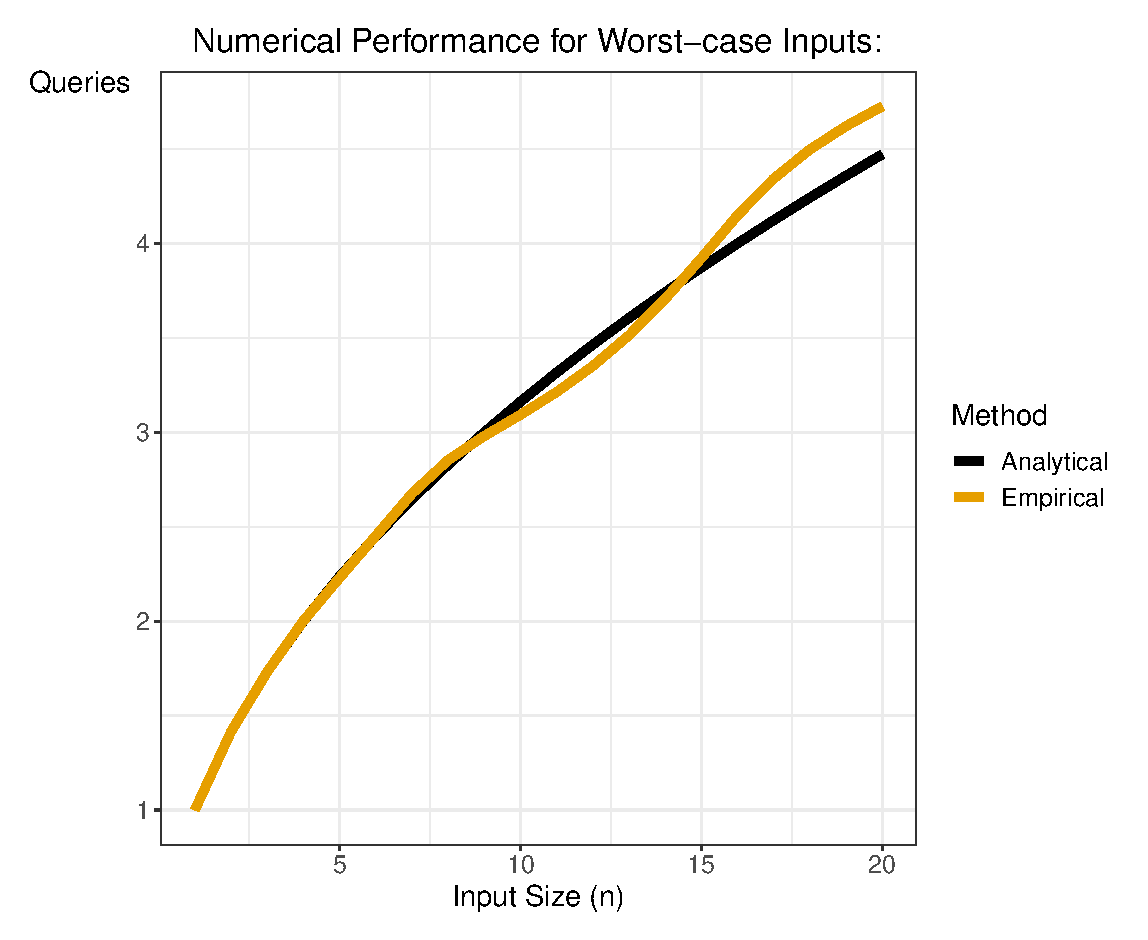
\includegraphics[scale=.5]{figure_worst_or_complexity}
\caption{The proven analytical optimal query complexity
and calculated empirical optimal query complexity by 
size of input bit string.}
\label{fig:or_worst_complexity}
\end{figure}

\begin{figure}[ht]
\centering
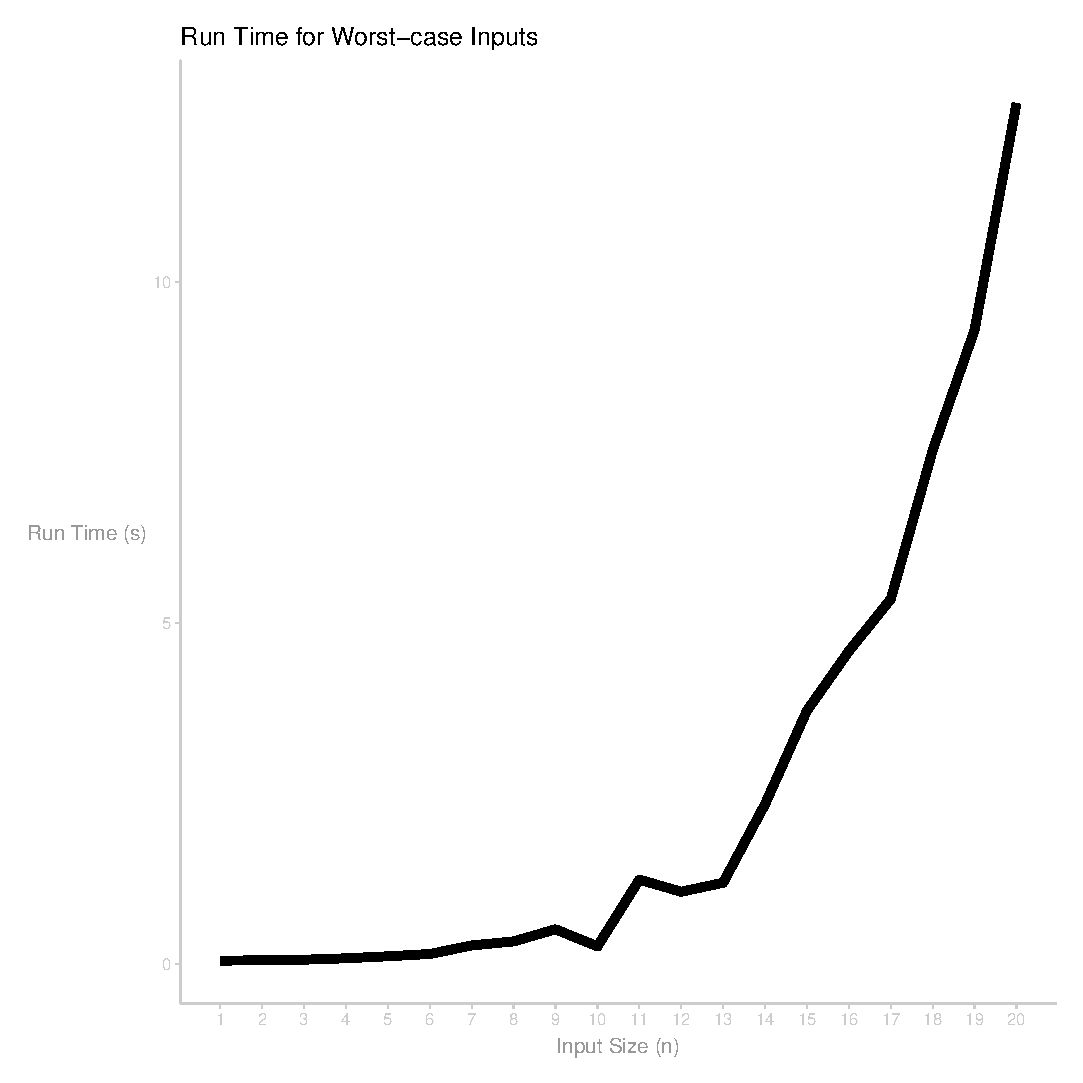
\includegraphics[scale=.4]{figure_worst_or_time}
\caption{Runtime of SDP solver by size of input strings.}
\label{fig:or_worst_runtime}
\end{figure}

The runtime is drastically improved over the all-case scenario. 
This result is not only show via the y-axis of the graphs, 
but also in the x-axis because the speed up was so 
significant that we were able to solve for many more 
input sizes than in the all-case scenario. 
Looking at the optimal query complexities returned, 
we observe that we are still obtaining good 
approximations of the true value. 
We believe that more iterations could drastically 
improve the performance of the algorithm as well as 
improved stopping conditions. Instead of simply stopping 
after some number of iterations (in this case 100), 
we could look to see if the improvements to the objective 
function are negligible and conclude that the algorithm has converged.
